\documentclass[../languages.tex]{subfiles}

\begin{document}
\usec{C}\label{sec:c}

\cd{C} is a general-purpose, imperative computer programming languages,
supporting structured programming, lexical variable scope and recursion, while a
static type system prevents many unintended operations. By design, \cd{C}
provides constructs that map efficiently to typical machine instructions, and
therefore it has found lasting use in applications that had formerly been
coded in assembly languages, including operation systems, as well as various
application software for computers ranging from supercomputers to embedded
systems.

\cd{C} was originally developed by Dennis Ritchie between 1969 and 1973 at
Bell Labs, and used to re-implement the Unix operation system. It has since becomes one of the most widely used programming languages of all time, with \cd{C} compilers from various vendors available for the majority of
existing computer architectures and operating systems. C has been standardized
by the American National Standards Institute (ANSI) since 1989 and subsequently
by the International Organization for Standardization (ISO).

\cd{C} is an imperative procedural language. It was designed to be compiled
using a relatively straightforward compiler, to provide low-level access to
memory, to provide language constructs that map efficiently to machine
instructions, and to require minimal run-time support. Despite its low-level
capabilities, the language was designed to encourage cross-platform
programming. A standards-compliant and portably written \cd{C} program can
be compiled for a very wide variety of computer platforms and operating systems
with few changes to its source code. The language has become available on a
very wide range of platforms, from embedded micro controllers to supercomputers.

\subsection{Influence}\label{sub:influence}

\begin{Figure}
  \centering
  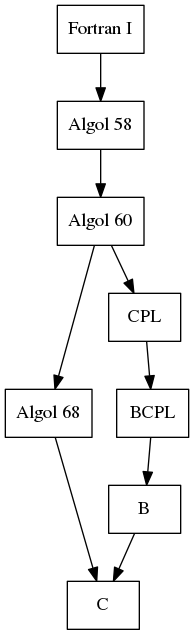
\includegraphics[height=0.5\textheight]{c}
  \captionof{figure}{Inheritance diagram for \cd{C}.}
\end{Figure}

\cd{C} was primarily influenced by the languages of \cd{B},
\cd{Algol}, \cd{Assembly}, and \cd{Fortran}.

\subsection{Hello World}
\label{sub:hello_world}

\begin{minted}[frame=lines]{c}
#include <stdio.h>

int main(void)
{
  printf("Hello, world!\n");
  return 0;
}
\end{minted}

\subsection{Syntax}
\label{sub:syntax}

\subsubsection{Basic Syntax}
\label{ssub:basic_syntax}

\paragraph{Semicolons}
\label{par:semicolons}

In \cd{C} the semicolon is a statement terminator. So every statement must be
ended with a semicolon.

\begin{minted}[frame=lines]{c}
printf("Hello, world!\n");
return 0;
\end{minted}

\paragraph{Comments}
\label{par:comments}

Comments begin with a \cd{/*} and end with a \cd{*/}.

\begin{minted}[frame=lines]{c}
/* A comment in C */
\end{minted}

\paragraph{Identifiers}
\label{par:identifiers}

Identifiers can start with any character A to Z, a to z, or \cd{\_}, and can be
followed by any characters that are not \cd{@}, \cd{\$}, \cd{\%}. The
identifiers are case sensitive.

\subsubsection{Data Types}
\label{ssub:data_types}

\paragraph{Basic Types}
\label{par:basic_types}

\subparagraph{Integer Types}
\label{spar:integer_types}

\begin{enumerate}
  \item[char] 1 byte, -128 to 127 or 0 to 255.
  \item[unsigned char] 1 byte, 0 to 255.
  \item[signed char] 1 byte, -128 to 127.
  \item[int] 2 or 4 bytes, -32,768 to 32,767 or -2,147,483,648 to 2,147,483,647
  \item[unsigned int] 2 or 4 bytes, 0 to 65,535 or 0 to 4,294,967,295
\end{enumerate}

\newpage
\end{document}
